

\PassOptionsToPackage{table}{xcolor} % to use colors in tables
\PassOptionsToPackage{pdfa}{hyperref}
\documentclass{unipd-thesis-modern} % src: https://github.com/baronefr/unipd-


% additional packages
\usepackage{amsmath}
\usepackage{lipsum} % for DEMO only
\usepackage{threeparttable}
\usepackage{threeparttable}
\usepackage{siunitx}
\usepackage[titles]{tocloft} % to modify spacing in toc chapters
\usepackage{tabularx}
\usepackage{booktabs}
\usepackage{caption}
\usepackage{array}
\usepackage[utf8]{inputenc}
\usepackage{titlesec} % Paquete para controlar espaciado de títulos
\usepackage{graphicx}
\usepackage{float} % para usar [H] si quieres fijar la figura

\setlength{\cftbeforechapskip}{7pt}
\setcounter{tocdepth}{4} % ToC depth

% titles
\title{Estimación de la Tasa de Pobreza en Colombia: Estimación de Área Pequeña Usando Modelos Mixtos y Componentes Espaciales}
\thesisHeader{Pontificia Universidad Javeriana Cali \\Facultad de Ingeniería y Ciencias.\\MAESTRÍA EN CIENCIA DE DATOS}
\academicYear{02-2026/06-2026}

% students
\author{Brayan Salgado Blanco \\Erick Caicedo Ruiz \\Juan Trochez Guayara
}

% supervisor(s)
\advisor{Sandra Milena Ramírez Buelvas}{Pontificia Universidad Javeriana} % (mandatory)
\coadvisor{Luis Fernando Aguado Quintero }{Pontificia Universidad Javeriana} 
% (optional, comment to remove)
%\otheradvisor{Prof. Paolino Paperino}{University of Padua} % (optional, comment to remove)
% ^ NOTE: you can use optional arg to customize the label "Internal Supervisor"
%   example:   \otheradvisor[The best supervisor!]{Prof. Paolino Paperino}{University of Padua}

% dedication (comment to remove)
\dedication{\textit{A nuestras familias y amigos\\}}

% custom symbols (optional)
\input{custom-symbols}

% bibliography file
\addbibresource{refs.bib}

\sisetup{
  output-decimal-marker = {.},
  group-separator = {,},
  detect-all = true
}


% Ajustes de espacio
\titlespacing*{\subsection}{0pt}{10pt plus 2pt minus 2pt}{5pt}
\titlespacing*{\subsubsection}{0pt}{5pt plus 2pt minus 2pt}{3pt}
% Otros paquetes y configuraciones
\setlength{\intextsep}{6pt}      % Espacio entre texto y figuras
\setlength{\textfloatsep}{6pt}   % Espacio entre texto y flotantes


\begin{document}
\renewcommand{\tablename}{Tabla}
\renewcommand{\listfigurename}{Lista de figuras}
\renewcommand{\listtablename}{Lista de tablas}
    \frontmatter
    % --------------------------
    \newpage
    \chapter{\textbf{INTRODUCCIÓN}}
La medición de la pobreza en Colombia enfrenta importantes desafíos derivados de la limitada
representatividad muestral de las encuestas de hogares y de la ausencia de información actualizada con
cobertura completa para todos los municipios del país. En el caso particular del Índice de Pobreza
Multidimensional (IPM), la última medición con alcance municipal proviene del Censo de 2018, lo que
genera un vacío significativo para el análisis territorial y la focalización de políticas públicas. Esta carencia dificulta identificar desigualdades persistentes, evaluar agendas como el avance en los Objetivos de Desarrollo Sostenible y orientar intervenciones sociales de manera precisa. \\

\setlength{\parindent}{2em} En este contexto, la estimación para áreas pequeñas (Small Area Estimation, SAE) se presenta como una alternativa metodológica adecuada para generar indicadores robustos en dominios con escasa o nula representatividad muestral. La posibilidad de integrar información censal, administrativa y muestral, así como de incorporar patrones de dependencia geográfica mediante modelos espaciales, permite formular estimaciones coherentes y territorialmente consistentes. Estas características hacen que la combinación de modelos SAE y enfoques espaciales sea especialmente pertinente para el caso colombiano, donde las brechas territoriales requieren instrumentos analíticos más finos y oportunos. \\

\setlength{\parindent}{2em} El proyecto se orienta a desarrollar una metodología estadística de estimación municipal del IPM que articule estas metodologías con el uso de fuentes oficiales del DANE y otras bases de datos
complementarias (también abiertas). Asimismo, se propone evaluar diferentes alternativas de modelamiento, contrastarlas a partir de criterios de coherencia geográfica y desempeño estadístico, y analizar los patrones territoriales que surjan del ejercicio. \\

\setlength{\parindent}{2em} En conjunto, esta propuesta busca contribuir a mejorar la disponibilidad de información para el diseño y focalización de políticas públicas, fortalecer el análisis territorial y aportar una herramienta metodológica replicable para el estudio de fenómenos sociales en contextos de baja representatividad estadística.
    \newpage
    % --------------------------
    \mainmatter
    % --------------------------
    \chapter{Definición del problema}
El presente proyecto se centra en abordar la falta de una metodología estadística validada que permita estimar la pobreza multidimensional con precisión y coherencia espacial a nivel municipal en Colombia. Este vacío metodológico se origina en la carencia de representatividad muestral de las encuestas oficiales como la Gran Encuesta Integrada de Hogares (GEIH) y la Encuesta Nacional de Calidad de Vida (ECV), las cuales están diseñadas para producir estimaciones departamentales o regionales, pero no locales \cite{DANE_ENCV_2022}. Esta limitación impide identificar desigualdades territoriales específicas y restringe la capacidad institucional para focalizar políticas públicas efectivas en municipios con alta vulnerabilidad socioeconómica \cite{CEPAL_PanoramaSocial_2023}.

Si la falta de estimaciones municipales precisas se mantiene, las implicaciones serán concretas y de alto impacto para la gestión pública: i) la asignación de recursos continuará guiándose por promedios departamentales, lo que puede ocultar diferencias relevantes entre municipios y dejar sin focalización adecuada a territorios altamente vulnerables; ii) programas sociales y proyectos de inversión podrían
seguir implementándose en zonas no prioritarias, reduciendo la eficacia y la eficiencia del gasto público;
y iii) la ausencia de información granular a nivel municipal limita la capacidad institucional de monitorear intervenciones, evaluar resultados y ajustar políticas basadas en evidencia. En conjunto, la falta de indicadores confiables a esta escala perpetúa decisiones menos informadas y debilita la capacidad del Estado para responder de manera diferenciada a los desafíos territoriales.

La definición del problema, por tanto, delimita su alcance a la esfera cuantitativa y metodológica del análisis estadístico, con un enfoque en el desarrollo, ajuste y evaluación de modelos SAE con dependencia espacial. El estudio se restringe al territorio colombiano y se aplicará de manera experimental sobre información proveniente de censos, encuestas y registros administrativos públicos.
De esta manera, se busca reducir la brecha de información a escala municipal y aportar una herramienta técnica que fortalezca la medición de la pobreza y la gestión pública basada en evidencia \cite{MolinaRao_2010} \cite{PratesiSalvati_2019} \cite{RaoMolina_2015}.
    
    \section{Planteamiento del problema}

En Colombia, la medición de la pobreza es un insumo crítico para el diseño, seguimiento y evaluación de las políticas públicas de bienestar social y equidad territorial. Este análisis se aborda mediante dos enfoques complementarios: la pobreza monetaria, que identifica a los hogares con ingresos insuficientes para adquirir una canasta básica de bienes y servicios, y la pobreza multidimensional, instrumentada a través del Índice de Pobreza Multidimensional (IPM), que evalúa privaciones estructurales en educación, salud, trabajo, niñez y vivienda. Mientras el primer enfoque examina la suficiencia de ingresos, el IPM captura las carencias materiales y de capacidades que afectan el bienestar de los hogares \cite{DANE_PobrezaMultidimensional_2023}.

No obstante, las estimaciones oficiales del Departamento Administrativo Nacional de Estadística (DANE) se desagregan, por lo general, a nivel departamental o para las principales áreas metropolitanas. Esta escala analítica diluye las heterogeneidades locales y oculta los contrastes socioeconómicos existentes entre municipios \cite{DANE_PobrezaMultidimensional_2023}. La ausencia de datos confiables a escala municipal debilita la focalización de programas sociales, la distribución eficiente de recursos y la formulación de políticas adaptadas a las realidades de las regiones históricamente rezagadas. La raíz del problema es metodológica: las encuestas de hogares empleadas para estas mediciones —como la Gran Encuesta Integrada de Hogares (GEIH) o la Encuesta Nacional de Calidad de Vida (ECV)— poseen diseños muestrales representativos a nivel departamental, pero carecen de la potencia estadística necesaria para realizar inferencias válidas en el ámbito municipal \cite{DANE_ENCV_2022}.

A esta restricción espacial se suma una limitación temporal. Colombia carece de mediciones oficiales directas y frecuentes del IPM municipal, lo que impide monitorear oportunamente la evolución de las privaciones en unidades territoriales pequeñas. Las estadísticas oficiales con mayor desagregación geográfica provienen de los censos de población y vivienda debido a su cobertura exhaustiva. Sin embargo, al ser operaciones periódicas y no anuales, los censos no permiten un seguimiento continuo. Este desfase intercensal genera un vacío de información que restringe la actualización del IPM municipal y reduce la capacidad institucional para detectar cambios recientes en las condiciones de vida de la población \cite{DANE_PobrezaMultidimensional_2023} \cite{DANE_ENCV_2022}.

Ante la inviabilidad de obtener mediciones directas actualizadas a nivel municipal, este proyecto implementa la estimación indirecta del IPM. En un entorno de alta desigualdad y heterogeneidad territorial como el colombiano, los promedios departamentales suelen enmascarar brechas críticas; dentro de un mismo departamento coexisten municipios con estándares de bienestar urbanos junto a otros con niveles de pobreza propios de las zonas rurales más vulnerables \cite{CEPAL_PanoramaSocial_2023}. Para resolver esta restricción, la estadística aplicada y la ciencia de datos ofrecen metodologías de Estimación para Áreas Pequeñas (Small Area Estimation, SAE), diseñadas para producir inferencias precisas en dominios con muestras insuficientes mediante la integración de múltiples fuentes de información \cite{RaoMolina_2015}.

Estos enfoques combinan los datos de encuestas con variables auxiliares procedentes de censos, registros administrativos o imágenes satelitales, empleando modelos jerárquicos o mixtos que incorporan estructuras espaciales \cite{MolinaRao_2010}. Al aprovechar la correlación geográfica entre unidades territoriales contiguas, estos modelos mejoran la precisión y la coherencia espacial de las estimaciones \cite{PratesiSalvati_2019}. En el contexto nacional, el uso de metodologías SAE se encuentra en desarrollo. Aunque estudios recientes demuestran su potencial para optimizar la medición de indicadores sociales a escala subnacional \cite{DANE_PobrezaMultidimensional_2023} \cite{LopezSanchezPerez_2021}, su aplicación al IPM sigue siendo incipiente. La adopción de modelos mixtos con componentes espaciales representa un avance metodológico clave para generar estimaciones consistentes, especialmente en municipios con baja representatividad muestral o registros administrativos deficientes.

La resolución de este problema técnico es indispensable para consolidar una gestión pública basada en evidencia, donde la disponibilidad de datos robustos a nivel municipal es el eje para optimizar la asignación presupuestal y formular políticas con precisión geoespacial \cite{PNUD_HDR_2022}. Desde la perspectiva de la ciencia de datos, el desafío radica en el desarrollo de arquitecturas analíticas capaces de integrar fuentes heterogéneas para mitigar la invisibilidad estadística de las comunidades más vulnerables, cuya situación socioeconómica suele quedar subrepresentada en los agregados oficiales.
    \newpage
    
\section{Formulación del problema}
¿Cómo estimar la tasa de pobreza multidimensional a nivel municipal en Colombia mediante modelos de estimación para áreas pequeñas con componentes espaciales, utilizando fuentes oficiales de datos del DANE?

Las preguntas de sistematización que apoyan la pregunta de formulación:

\begin{enumerate}
    \item ¿Cómo incorporar componentes espaciales en los modelos de estimación para áreas pequeñas con el fin de capturar la correlación geográfica entre municipios y mejorar la precisión y robustez de las estimaciones de pobreza multidimensional?

    \item ¿Cuáles son las variables más relevantes, según los modelos de área pequeña, para explicar la pobreza multidimensional a nivel municipal en Colombia, entre las disponibles en las fuentes oficiales de datos del DANE?

    \item ¿Qué patrones espaciales se observan en la distribución estimada de la pobreza multidimensional municipal a partir de los modelos de área pequeña?
\end{enumerate}

    % --------------------------
    \chapter{Objetivos del proyecto} % 
    \section{Objetivo general}
Desarrollar una metodología de estimación para áreas pequeñas con componentes espaciales que permita estimar la tasa de pobreza multidimensional a nivel municipal en Colombia, a partir de fuentes oficiales de información del DANE.

    \section{Objetivos específicos}

\begin{enumerate}
    \item Evaluar el desempeño de modelos de estimación para áreas pequeñas (SAE) que incorporen componentes espaciales, determinando su capacidad para capturar la correlación geográfica intermunicipal y optimizar la precisión del IPM en zonas con baja representatividad muestral.

    \item Identificar, mediante los modelos seleccionados, las variables auxiliares provenientes de las fuentes oficiales del DANE con mayor poder explicativo sobre la pobreza multidimensional a escala municipal.

    \item Caracterizar la distribución y las estructuras de dependencia espacial de la pobreza multidimensional municipal a partir de las estimaciones indirectas generadas.
\end{enumerate}



    % --------------------------
    \chapter{Marco de referencia}
El estudio de la pobreza desde una perspectivaerritorial exige bases conceptuales y metodológicas que permitan comprender tanto la naturaleza multidimensional del fenómeno como los desafíos asociados a su medición en escalas geográficas pequeñas. En particular, la combinación de encuestas de hogares con fuentes censales y registros administrativos abre la posibilidad de utilizar metodologías estadísticas avanzadas que compensen la falta de representatividad muestral en dominios territoriales pequeños.

Este capítulo presenta los fundamentos teóricos que sustentan el uso de técnicas de Estimación para Áreas Pequeñas (Small Area Estimation, SAE), sus extensiones espaciales y los aportes recientes de la ciencia de datos para el análisis territorial de la pobreza. Además, se integran antecedentes relevantes que demuestran el uso y la pertinencia de estas metodologías en América Latina y Colombia.
    %--------------------------------------------------
\section{MARCO TEÓRICO}
La pobreza multidimensional reconoce que las privaciones que enfrentan los hogares trascienden el ingreso e incluyen dimensiones como salud, educación, vivienda, servicios básicos y empleo. En Colombia, su medición oficial se realiza mediante el Índice de Pobreza Multidimensional (IPM), lo que permite identificar privaciones específicas y orientar intervenciones focalizadas. Sin embargo, la disponibilidad territorial del IPM es limitada: salvo la estimación derivada del Censo 2018, no existen mediciones periódicas para los 1.122 municipios del país. Esta brecha de información dificulta el diagnóstico local y la formulación de políticas basadas en evidencia, especialmente en zonas con baja representatividad estadística. Este vacío metodológico motiva el uso de técnicas capaces de producir estimaciones confiables a nivel municipal mediante fuentes auxiliares, como la Estimación para Áreas Pequeñas (SAE).

Los modelos SAE ofrecen una base estadística sólida para generar estimaciones precisas en dominios con escasa muestra, mediante la integración de información proveniente de censos, registros
administrativos y encuestas \cite{CEPAL_PovertyMapping_2022}. Existen dos grandes enfoques: los modelos de área, como el modelo
Fay–Herriot, que utilizan estimaciones directas agregadas y covariables auxiliares; y los modelos de unidad, que emplean microdatos para capturar variabilidad individual. La selección depende de la calidad y granularidad de las fuentes disponibles, pero ambos enfoques permiten mejorar la precisión, reducir la varianza y generar estimaciones territorialmente consistentes, lo cual es fundamental en contextos municipales.

No obstante, cuando los indicadores presentan patrones territoriales no explicados completamente por las covariables, resulta necesarioenfoques espaciales que modelen explícitamente la dependencia geográfica. Los modelos espaciales integran estructuras de vecindad o efectos aleatorios espaciales, lo que permite “suavizar” las estimaciones entre municipios contiguos y reducir variabilidad no explicada. La literatura demuestra que estos modelos mejoran la coherencia territorial, especialmente en dominios pequeños y heterogéneos como los municipios colombianos \cite{PratesiSalvati_2019}.

Las herramientas de ciencia de datos complementan este proceso al facilitar la selección de variables auxiliares, el análisis de relaciones no lineales y la integración de datos heterogéneos, incluyendo fuentes satelitales como VIIRS. Asimismo, la visualización interactiva (a través de dashboards y mapas
temáticos) constituye un elemento clave para la interpretación y difusión de resultados, permitiendo a instituciones y tomadores de decisión explorar patrones territoriales de manera más accesible.

La aplicación de modelos SAE y de sus extensiones espaciales depende directamente de la disponibilidad de covariables confiables y de cobertura completa. En este proyecto se emplearán fuentes oficiales como el Censo Nacional de Población y Vivienda 2018, la GEIH y la ECV del DANE, registros administrativos sectoriales y datos geoespaciales abiertos. A partir de estas fuentes se derivarán variables relacionadas con condiciones de vivienda, servicios públicos, educación, entorno e infraestructura, esenciales para mejorar la capacidad predictiva del modelo y compensar la baja representatividad muestral en muchos
municipios.

En conjunto, los enfoques revisados —modelos SAE, modelos espaciales, herramientas de ciencia de datos y visualización— constituyen el fundamento conceptual que sustenta este proyecto. Su
integración permite generar estimaciones municipales del IPM más precisas y territorialmente coherentes, aportando una base metodológica adecuada para el análisis territorial en contextos con
limitaciones de información estadística.

%--------------------------------------------------
%\section{Fundamento teórico de ciencia de datos}
%\label{sec:Fundamento-teorico}

%    %--------------------------------------------------
%    \subsection{Modelo 1}

 %   \begin{equation}
 %   \begin{aligned}
 %       \operatorname{Bin}(y_i \mid n_i, \theta_i)
 %       &\propto \theta_i^{y_i} (1 - \theta_i)^{n_i - y_i} \\
 %       &\propto \exp(\eta_{i 1})^{y_i} / (1 + \exp(\eta_{i 1}))^{n_i} \\
 %       &\propto (e^\psi)^a / (1 + e^\psi)^b
 %   \end{aligned}
 %   \label{eq:binomial-likelihood}
 %   \end{equation}
    
    
 %   %--------------------------------------------------
 %   \subsection{Modelo 2}
    
    
    
    % \begin{figure}[!htbp]
    %     \centering
    %     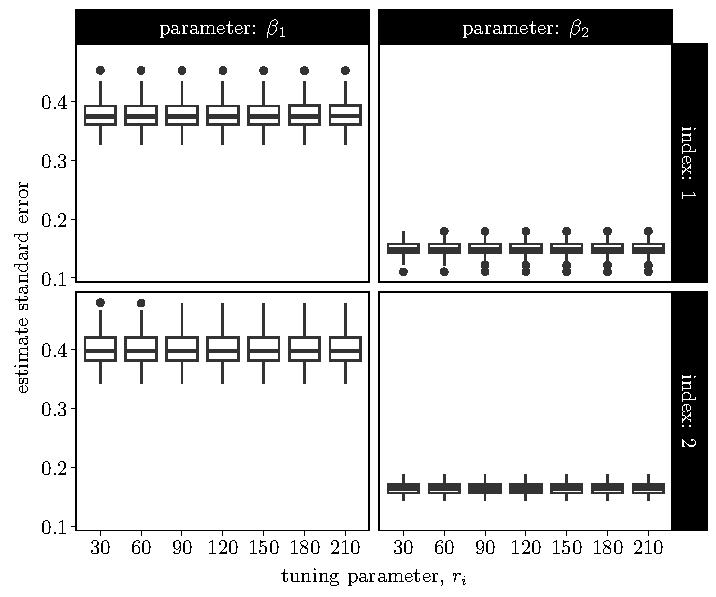
\includegraphics[width=0.75\textwidth]{fig/fig_new_experiment_01.pdf}
    %     \caption{Estimate standard errors as a function of the tuning parameter $r_i$. The standard errors are relatively stable across values of $r_i$.}
    %     \label{fig:fig_new_exp_01}
    % \end{figure}
    \section{Antecedentes}
\label{sec:antecedentes}
La formulación de políticas públicas contemporáneas opera bajo el mandato global de \textit{``No dejar a nadie atrás''} (\textit{Leave No One Behind}, LNOB), eje transversal de la Agenda 2030 para el Desarrollo Sostenible \cite{cepal2024, un2030}. Este compromiso internacional ha impulsado una transición analítica desde los agregados nacionales hacia una mayor granularidad subnacional, reconociendo que los promedios macroeconómicos suelen disimular disparidades territoriales críticas. En este escenario, la Estimación en Áreas Pequeñas (\textit{Small Area Estimation}, SAE) surge como un paradigma metodológico indispensable para superar las limitaciones de representatividad de las encuestas de hogares, permitiendo fundamentar la intervención estatal en inferencias precisas a nivel municipal y local \cite{cepal2024, dane2024}.

\subsection{Evolución de la medición de pobreza y el desafío de la desagregación territorial}

Los paradigmas de medición de la pobreza han transitado de enfoques estrictamente monetarios hacia marcos multidimensionales basados, principalmente, en la metodología de Alkire y Foster \cite{alkire2011}. Este enfoque constituye la base técnica de diversos índices oficiales y sustenta ejercicios aplicados como el Índice de Pobreza Energética Multidimensional (IMPE) en Colombia, cuya implementación busca trasladar el análisis desde una perspectiva nacional hacia una escala municipal, idónea para identificar brechas estructurales en zonas rurales dispersas \cite{promigas2025}.

No obstante, la generación de estas estadísticas enfrenta un obstáculo inferencial persistente: las encuestas de hogares tradicionales ---como la Pesquisa Nacional por Amostra de Domicílios Contínua (PNADC) en Brasil o la Gran Encuesta Integrada de Hogares (GEIH) en Colombia--- están diseñadas para ofrecer representatividad en dominios geográficos mayores. Por tanto, al desagregar los datos para municipios o estratos territoriales pequeños, la varianza y los errores de muestreo se incrementan sustancialmente, invalidando las estimaciones directas \cite{moura2021, dane2024}.

Según la documentación técnica del Departamento Administrativo Nacional de Estadística (DANE), la arquitectura estadística en Colombia padece una marcada asimetría temporal y geográfica. Mientras el nivel departamental cuenta con una periodicidad anual respaldada por encuestas continuas, la información municipal depende de censos nacionales realizados cada diez o quince años \cite{dane2024}. Este desfase intercensal genera un vacío de información que obstruye el monitoreo oportuno de las metas de desarrollo. Ante esta restricción, la integración de encuestas de alta periodicidad con registros administrativos e información auxiliar se convierte en una condición necesaria para mantener la vigencia de las estadísticas oficiales y garantizar decisiones basadas en evidencia contemporánea.

\subsection{Modelos de estimación en áreas pequeñas en el contexto latinoamericano}

En América Latina, la Comisión Económica para América Latina y el Caribe (CEPAL) ha liderado la transferencia de metodologías SAE, priorizando modelos a nivel de unidad como el \textit{Empirical Best Predictor} (EBP) y el \textit{Pseudo-EBP} \cite{cepal2024}. Este último resulta crucial por su capacidad para incorporar los pesos de muestreo en el modelado, mitigando el sesgo derivado de ignorar el diseño complejo de las encuestas. Estos enfoques articulan la precisión analítica de los datos muestrales con la cobertura exhaustiva de los censos y otras fuentes auxiliares, incluyendo sensores remotos.

Dentro de las experiencias regionales, Brasil constituye un referente metodológico relevante mediante el desarrollo de modelos SAE bajo distribución Beta con función de enlace logística para estimar la incidencia, el hiato y la severidad de la pobreza \cite{moura2021}. Las aplicaciones basadas en la PNADC demuestran que la inclusión de series históricas de al menos cuatro años en estructuras temporales estabiliza y mejora significativamente la precisión frente a los estimadores directos, alcanzando estándares de calidad aptos para la publicación oficial.

A este ecosistema metodológico se suma la incorporación de variables auxiliares geoespaciales. Plataformas como Google Earth Engine facilitan la extracción de predictores robustos ---luces nocturnas, cobertura urbana o índices de vegetación--- a partir de imágenes satelitales como Sentinel-2 y PlanetScope \cite{cepal2024, dane2024}. Estas variables operan como indicadores indirectos (*proxies*) de la actividad económica y el bienestar en territorios con registros administrativos deficientes. Así, la integración de componentes espaciales y fuentes alternas reduce la dependencia de censos desactualizados frente a dinámicas territoriales aceleradas, como la expansión urbana o las transformaciones agrícolas.

\subsection{Avances y experiencias de aplicación en Colombia}

En el ámbito nacional, el DANE ha avanzado en la implementación de modelos de área de tipo Fay-Herriot, aplicados a la Encuesta Nacional de Demografía y Salud (ENDS 2015) para estimar la proporción de hogares con miembros en el extranjero \cite{dane2024}. Asimismo, la entidad evalúa modelos mixtos generalizados con componentes geoestadísticos para el mapeo subnacional de la pobreza monetaria. Aunque estos desarrollos denotan un progreso técnico importante, su consolidación metodológica y difusión pública permanecen en fase de validación.

Por otra parte, el sector privado ha aportado análisis territoriales sobre privaciones multidimensionales. El reporte del IMPE 2025 de Promigas, por ejemplo, cartografía la denominada \textit{periferia energética} en departamentos como Chocó, La Guajira y Vichada \cite{promigas2025}. Los hallazgos revelan que la pobreza energética en zonas rurales remotas supera críticamente a la de los centros urbanos. Frente a este panorama, el informe define metas de reducción del indicador y propone líneas de acción concretas, tales como la optimización del servicio eléctrico, la sustitución de leña, la digitalización del hogar y la electrificación de instituciones educativas.

En el plano tecnológico, el DANE ha incorporado algoritmos de *Machine Learning* como Random Forest y XGBoost para la clasificación supervisada de coberturas vegetales y la actualización de marcos muestrales agropecuarios \cite{dane2024}. Estas innovaciones responden a la exigencia del Plan Nacional de Desarrollo 2022--2026 de producir estadísticas oficiales más desagregadas para visibilizar a grupos históricamente excluidos.

\subsection{Vacíos en la literatura y justificación metodológica}

A pesar de las iniciativas descritas, la estimación de la pobreza multidimensional a nivel municipal mediante modelos mixtos complejos con componentes espaciales sigue siendo un campo en consolidación \cite{dane2024}. Si bien se registran avances en pobreza monetaria y metodologías SAE generales, Colombia aún no dispone de un protocolo estandarizado, validado y publicado para la estimación anualizada de la pobreza multidimensional municipal a partir de las fuentes del DANE.

La literatura identifica, además, desafíos persistentes en la integración de datos. Destacan el sesgo de enlace (*linking bias*), asociado a las dificultades operativas en el cruce de encuestas y registros administrativos, y la cobertura incompleta de estos últimos. Asimismo, se evidencia una ausencia de protocolos consolidados para la homologación de categorías, variables y formatos entre las distintas fuentes de información \cite{dane2024}, lo que compromete la consistencia de los modelos y limita la comparabilidad local.

Ante la inexistencia de una metodología oficial estandarizada para evaluar anualmente el IPM municipal, esta propuesta resulta plenamente justificada. El desarrollo de una estrategia de estimación para áreas pequeñas con componentes espaciales permitirá mitigar el vacío de información intercensal y estructurar un monitoreo sistemático de los riesgos y desigualdades territoriales, proveyendo un insumo robusto para el diseño de políticas públicas focalizadas.
    % --------------------------
    \chapter{Datos}
        La etapa de preprocesamiento comprende la construcción, depuración y armonización de los datos que sustentarán el modelado de Estimación para Áreas Pequeñas (SAE) con componente espacial. Este procedimiento integra encuestas y registros administrativos en estructuras territoriales coherentes, garantizando la trazabilidad mediante llaves geográficas estandarizadas (códigos DANE de departamento y municipio) y unificando definiciones, periodos de referencia y unidades de análisis.

Bajo este esquema, se calculó el Índice de Pobreza Multidimensional (IPM) 2024 a nivel departamental utilizando la Encuesta Nacional de Calidad de Vida (ECV) 2024. Esta estimación directa opera como la "verdad parcial" del ejercicio y, junto con sus varianzas asociadas —calculadas como el cuadrado del error estándar por dominio—, funciona como el anclaje metodológico del enfoque SAE.

En paralelo, se consolidó una matriz de covariables auxiliares a escala municipal a partir de registros administrativos y fuentes oficiales complementarias. Esta matriz agrupa variables vinculadas a condiciones estructurales de salud, educación e infraestructura básica, seleccionadas bajo criterios de disponibilidad territorial, pertinencia conceptual y capacidad explicativa respecto a la pobreza multidimensional. La estructura y el detalle de estos predictores se describen en la Tabla 4.1.

\begin{table}[H]
\centering
\small
\caption{Variables identificadoras y covariables auxiliares de la matriz municipal para la estimación del IPM 2024}
\label{tab:matriz-auxiliar-ipm}
\renewcommand{\arraystretch}{1.25}
\begin{tabular}{p{4.2cm} p{2.6cm} p{6.2cm}}
\hline
\textbf{Variable} & \textbf{Bloque} & \textbf{Descripción} \\
\hline
Código DANE del departamento & Identificación territorial & Código oficial DANE del departamento. \\
Nombre del departamento & Identificación territorial & Nombre del departamento. \\
Código DANE del municipio & Identificación territorial & Código oficial DANE del municipio. \\
Nombre del municipio & Identificación territorial & Nombre del municipio. \\
Porcentaje de afiliados al régimen subsidiado (2024) & Salud & Porcentaje de afiliados al régimen subsidiado en 2024. \\
Porcentaje de afiliados al régimen contributivo (2024) & Salud & Porcentaje de afiliados al régimen contributivo en 2024. \\
Aseguramiento en salud ajustado o capado (2024) & Salud & Cobertura total de aseguramiento en salud ajustada mediante truncamiento superior. \\
Razón subsidiado/contributivo (2024) & Salud & Razón entre afiliados al régimen subsidiado y contributivo. \\
Logaritmo del total de afiliados en salud (2024) & Salud & Logaritmo natural del total de afiliados al sistema de salud. \\
Tasa de matriculación de 5 a 16 años & Educación & Tasa de matriculación de la población entre 5 y 16 años. \\
Cobertura neta educativa total & Educación & Cobertura neta total del sistema educativo. \\
Cobertura neta en educación media & Educación & Cobertura neta en educación media. \\
Tasa de deserción escolar & Educación & Tasa de deserción escolar. \\
Tasa de repitencia escolar & Educación & Tasa de repitencia escolar. \\
Tasa de reprobación escolar & Educación & Tasa de reprobación escolar. \\
Cobertura de acueducto & Infraestructura básica & Cobertura municipal del servicio de acueducto. \\
Cobertura de alcantarillado & Infraestructura básica & Cobertura municipal del servicio de alcantarillado. \\
Cobertura de aseo & Infraestructura básica & Cobertura municipal del servicio de aseo. \\
Índice de infraestructura básica & Infraestructura básica & Índice compuesto calculado como el promedio simple de acueducto, alcantarillado y aseo. \\
Cobertura de energía rural & Infraestructura básica & Cobertura de energía eléctrica en zona rural. \\
\hline
\end{tabular}
\end{table}
\noindent \textit{Nota.} Las variables de identificación territorial no operan como predictores en el modelo, sino como llaves de integración, validación y representación cartográfica. \\

El control de calidad de la información incluyó la verificación de la consistencia interna, la unicidad de los registros municipales, la correspondencia del codigoficado DANE, la identificación de valores faltantes y la detección de coberturas atípicas. Particularmente en el bloque de salud, se diseñó un indicador de aseguramiento ajustado mediante truncamiento superior para corregir registros de cobertura nominalmente mayores al 100\%. Asimismo, se aplicaron transformaciones logarítmicas al total de afiliados para mitigar asimetrías y estabilizar el comportamiento del modelo.

En el componente de infraestructura básica, se estimó un indicador sintético a partir del promedio simple de las coberturas de acueducto, alcantarillado y aseo. Por su parte, la cobertura de energía rural se preservó como una covariable independiente para evaluar de manera aislada su contribución durante la fase de selección de predictores.

Para armonizar las escalas de análisis, las covariables de la matriz municipal se agregaron a nivel departamental mediante promedios simples. Esto permitió estructurar una base analítica departamental de 33 observaciones, correspondiente a los dominios con estimación directa del IPM y varianza calculada. El cruce entre la estimación directa y la matriz auxiliar agregada se ejecutó mediante el código DANE departamental, mitigando inconsistencias por variaciones en la nomenclatura textual de las regiones. La base final resultante presenta una cobertura casi exhaustiva, registrando un único dato faltante en la variable de cobertura de aseo.

Al cierre de esta etapa se dispuso de la base de estimación directa de la ECV 2024 con sus varianzas, la matriz municipal de covariables y la base departamental integrada, listas para el análisis exploratorio y la especificación del modelo. Los insumos geoespaciales —*shapefile* municipal y matriz de vecindad— se acoplarán posteriormente al activar el componente espacial del estimador SAE.

Con la base analítica consolidada, el paso siguiente consistió en evaluar el potencial explicativo de las covariables. El análisis exploratorio subsiguiente se orientó a examinar la asociación entre estos predictores y el IPM departamental directo, buscando el equilibrio entre consistencia teórica, estabilidad estadística y parsimonia. Dado que este proceso fundamenta la estrategia analítica del modelo y trasciende la descripción de las fuentes, su desarrollo formal se detalla en el capítulo de Metodología.
    % --------------------------
    \chapter{Metodología}
        %--------------------------------------------------
A partir de los antecedentes descritos, y considerando las limitaciones metodológicas identificadas en la
literatura, el presente proyecto incorpora un conjunto de orientaciones metodológicas preliminares que
fundamentan la elección de los modelos a emplear y la forma en que se evaluará su desempeño.

En este sentido, la metodología se estructura en función de los objetivos específicos del proyecto y se desarrolla mediante un conjunto de actividades organizadas de forma secuencial, desde la identificación de fuentes de información hasta el diseño, evaluación y análisis de los modelos de Estimación para Áreas Pequeñas (SAE) con componentes espaciales.

El diseño metodológico se estructura como una secuencia secuencial de preparación, evaluación y modelación estadística orientada a estimar el Índice de Pobreza Multidimensional (IPM) 2024 en escalas territoriales desagregadas mediante técnicas de estimación para áreas pequeñas (SAE). El flujo operativo comprende la depuración y armonización de fuentes, el diagnóstico de completitud, la construcción de bloques analíticos de covariables, la validación por especificaciones competitivas y el ajuste del modelo de áreas de Fay-Herriot. El proceso culmina con una evaluación crítica de la capacidad predictiva sintética a nivel municipal.

\subsection{Limpieza, filtrado y reglas explícitas}
La fase inicial consistió en la depuración y alineación geométrica de dos insumos complementarios: la estimación directa del IPM 2024 departamental con sus respectivas varianzas de muestreo, y la matriz de covariables auxiliares de cobertura municipal. En ambas fuentes se auditó la arquitectura de los archivos, la tipología de las variables y la integridad de los códigos divisionales del territorio.

La base departamental consolida los 33 dominios institucionales (32 departamentos y Bogotá D.C.). Al contener registros exclusivos del IPM 2024 para el subdominio geográfico «Total», el archivo prescindió de filtros temporales o geográficos adicionales y asumió la función de vector observado para la calibración del modelo. Por su parte, la matriz municipal abarca 1.122 observaciones, cuyas variables de identificación político-administrativa se estandarizaron bajo la codificación oficial del DANE (\texttt{\detokenize{cod_depto}}), (\texttt{\detokenize{cod_mpio}}), (\texttt{depto}), (\texttt{mpio}). Dentro de esta matriz se homogeneizó la nomenclatura del bloque de infraestructura (\texttt{\detokenize{Cobertura_acueducto}}), (\texttt{\detokenize{Cobertura_alcantarillado}}), (\texttt{\detokenize{Cobertura_aseo}}) y (\texttt{\detokenize{Cobertura_energia_rural}}) para corregir discrepancias de formato y asegurar la consistencia del procesamiento en bloque.

Como regla explícita de integración, el enlace de las bases se ejecutó estrictamente mediante el código numérico departamental (\texttt{\detokenize{cod_depto}}). Se descartó el uso de cadenas de texto debido a heterogeneidades de escritura en dominios como Valle del Cauca o el Archipiélago de San Andrés, Providencia y Santa Catalina, garantizando así un acoplamiento exacto y sin pérdida de registros. 

En el bloque sectorial de salud, la variable de aseguramiento se sometió a un truncamiento superior para neutralizar las inconsistencias derivadas de coberturas nominales superiores al 100\%. Asimismo, se introdujo la tasa de mortalidad infantil junto a su transformación logarítmica, calculada mediante $\log(1 + \text{mortalidad\_infantil})$, con el fin de corregir la asimetría distributiva de la variable y capturar de forma más robusta la vulnerabilidad sanitaria del dominio.

\subsection{Identificación de datos faltantes}
Sincronizadas las fuentes, se evaluó la completitud de la matriz municipal y de la estructura agregada departamental. A nivel municipal, el diagnóstico buscó vacíos de información en las dimensiones de servicios públicos e infraestructura. Tras consolidar los indicadores municipales a la escala de calibración, la base analítica integrada presentó una cobertura exhaustiva en casi la totalidad de sus celdas. 

La única excepción fue (\texttt{cobertura\_aseo}), que registró un único dato faltante entre los 33 dominios. Al tratarse de una omisión aislada y dado que el atributo no demostró un rol crítico en las ecuaciones finales, se prescindió de algoritmos de imputación artificial. La estrategia optó por restringir los modelos definitivos —tanto el principal como el de sensibilidad— a covariables con soporte empírico pleno.

\subsection{Ventanas temporales y estrategia de validación}
El horizonte analítico del estudio se restringe de forma estricta al año 2024. Tanto el vector de respuesta (IPM directo departamental) como los bloques de información auxiliar coinciden en este periodo de referencia, asegurando que los coeficientes estimados describan vínculos contemporáneos del fenómeno.

A diferencia de los esquemas convencionales de aprendizaje supervisado, el modelado SAE no recurre a una partición de la muestra en conjuntos de entrenamiento y prueba. Esta decisión responde a la naturaleza del problema: el objetivo no radica en optimizar la predicción general fuera de muestra sobre un volumen masivo de observaciones independientes, sino en estabilizar y calibrar los parámetros de un modelo de áreas a partir de un número limitado de dominios observados para, posteriormente, extrapolar dicha relación a la escala municipal. 

Por lo tanto, el protocolo de validación se desplaza hacia el análisis de sensibilidad y la confrontación de especificaciones competitivas. El diseño evalúa un modelo principal y uno de sensibilidad; ambos integran tres covariables y difieren únicamente en la representación de la salud, alternando entre la escala natural de la mortalidad infantil y su aproximación logarítmica.

\subsection{Construcción de variables predictoras}
La matriz de predictores auxiliares se estructuró en tres dimensiones: salud, educación e infraestructura básica. Los criterios de inclusión exigieron cobertura territorial exhaustiva, sincronía con el año de referencia y pertinencia conceptual respecto a las privaciones constitutivas de la pobreza multidimensional.

\begin{itemize}
    \item \textbf{Salud}: Consolida el porcentaje de afiliados al régimen subsidiado (\texttt{pct\_subsidiado\_2024}), el porcentaje en el régimen contributivo (\texttt{pct\_cont\_2024}), el aseguramiento con truncamiento superior (\texttt{aseguramiento\_capado\_2024}), la razón subsidiado/contributivo (\texttt{ratio\_subs\_cont\_2024}), el logaritmo de la afiliación total (\texttt{log\_total\_afiliados\_2024}), la tasa de mortalidad infantil (\texttt{mortalidad\_infantil}) y su variante logarítmica (\texttt{log\_mortalidad\_infantil}). Estos indicadores operan como aproximaciones del acceso al sistema de protección y del rezago sanitario estructural.

    
    \item \textbf{Educación}: Incluye la tasa de matriculación en el rango de 5 a 16 años, la cobertura neta total, la cobertura neta en educación media, y las tasas de deserción, repitencia y reprobación. El bloque describe las trayectorias de permanencia y éxito escolar, ligadas directamente a las dimensiones de capital humano del índice.
    
    \item \textbf{Infraestructura básica}: Incorpora las coberturas individuales de acueducto, alcantarillado y aseo, junto con el indicador sintético (\texttt{infraestructura\-\_basica}) (definido como el promedio simple de las tres coberturas previas). Se aisló la cobertura de energía rural como predictor independiente para evaluar su comportamiento específico como vector de vulnerabilidad rural.
\end{itemize}

Estas variables se calcularon originalmente en la escala municipal. Para compatibilizarlas con el nivel de agregación de la encuesta, se sintetizaron a escala departamental mediante promedios aritméticos simples. La matriz auxiliar resultante cuenta con 33 observaciones y 21 columnas, incorporando el volumen de municipios por departamento como un descriptor del tamaño del dominio.

\subsection{Construcción de la variable respuesta}
El vector de respuesta corresponde al IPM directo departamental extraído de la Encuesta Nacional de Calidad de Vida (ECV) 2024. Este dato representa la «verdad parcial» del proceso, al constituir el nivel geográfico con estimaciones empíricas observables y errores de muestreo medibles. 

Cada estimación se emparejó con su varianza de muestreo (\texttt{vardir}), deducida del cuadrado del error estándar del dominio. En la arquitectura de Fay-Herriot, este parámetro es indispensable para balancear el nivel de confianza entre la estimación directa de la encuesta y la predicción basada en variables auxiliares. Aunque el fin último es inferir el IPM municipal, la calibración se ejecuta necesariamente en la escala departamental debido a la disponibilidad de estas varianzas de diseño; así, el nivel departamental actúa como espacio de entrenamiento lineal y el municipal como escala de proyección sintética.

\subsection{Análisis exploratorio}
Integrada la base analítica departamental, se evaluó la estructura de asociación bivariada entre el IPM directo y las covariables. Las correlaciones preliminares ratificaron el poder explicativo de la repitencia escolar y la relevancia de los bloques de infraestructura y salud en el comportamiento del indicador.

Antes del ajuste formal del modelo SAE, se estimaron ecuaciones lineales por mínimos ordinarios para evaluar combinaciones de variables. La selección de los predictores finales no dependió exclusivamente del valor p individual; se primó la coherencia de los signos teóricos, la estabilidad de los vectores de coeficientes, la parsimonia de la ecuación y el sustento conceptual de los atributos. 

La inclusión de la mortalidad infantil incrementó sustancialmente la capacidad explicativa general. El modelo que asocia las variables \texttt{repitencia}, \texttt{infraestructura\_basica} y \texttt{mortalidad\_infantil} registró un $R^2$ ajustado de 0,7537, con valores de $\text{AIC} = 227,64$ y $\text{BIC} = 235,13$, superando las alternativas basadas en la formalidad laboral (\texttt{pct\_cont\_2024}) y los modelos restrictivos de dos covariables. La alternativa con \texttt{log\_mortalidad\_infantil} mostró un ajuste aceptable ($R^2$ ajustado = 0,7106), aunque inferior a la tasa en escala original. Ensayos con la variable \texttt{pct\_cont\_2024} arrojaron coeficientes con el signo esperado, pero sin significancia estadística ni mejoras en los criterios de información, motivando su exclusión.

\subsection{Preprocesamiento específico para la modelación}
Con base en el comportamiento empírico del análisis exploratorio, se aislaron dos matrices específicas para el ajuste del modelo SAE. La primera, estructurada para la especificación principal, acopla los vectores (\texttt{ipm\_directo}), (\texttt{vardir}), (\texttt{repitencia}), (\texttt{infraestructura\_basica}) y (\texttt{mortalidad\_infantil}), junto con las llaves territoriales. La segunda matriz, destinada al análisis de sensibilidad, replica esta estructura pero sustituye la mortalidad infantil por su transformación logarítmica. En ambas bases se constató la ausencia de celdas vacías para las 33 unidades departamentales, garantizando matrices de entrada alineadas y libres de distorsiones de escala o cobertura.

\subsection{Especificación del modelo SAE}
La estimación de los parámetros se realizó mediante un modelo de áreas de Fay-Herriot, empleando el método de máxima verosimilitud restringida (REML). Se definieron dos ecuaciones funcionales.

La especificación adoptada como modelo principal se define como:
\begin{equation}
    \begin{split}        
        \text{IPM}_d^{\text{dir}} = {} & \beta_0 + \beta_1 \text{repitencia}_d + \beta_2 \text{infraestructura\_basica}_d \\ 
        & + \beta_3 \text{mortalidad\_infantil}_d + u_d + e_d
    \end{split}
\end{equation}

donde $\text{IPM}_d^{\text{dir}}$ es la estimación directa de la encuesta en el departamento $d$, $u_d$ representa el efecto aleatorio del área y $e_d$ el error de muestreo condicionado a la varianza de diseño conocida.

La ecuación para el análisis de sensibilidad formaliza el siguiente comportamiento:

\begin{equation}
    \begin{split}        
        \text{IPM}_d^{\text{dir}} = \beta_0 + \beta_1 \text{repitencia}_d + \beta_2  \text{infraestructura\_basica}_d  \\ + \beta_3 \text{log\_mortalidad\_infantil}_d + u_d + e_d
    \end{split}
\end{equation}

El modelo principal se seleccionó por exhibir un balance óptimo entre bondad de ajuste estadístico y parsimonia. La alternativa de sensibilidad se preservó exclusivamente como contraste para evaluar la estabilidad de las estimaciones ante cambios en la especificación funcional de la dimensión salud.

\subsection{Comparación de especificaciones y análisis de robustez}
Ambos algoritmos convergieron en cinco iteraciones, generando estimaciones lineales insesgadas óptimas empíricas (EBLUP) para la totalidad de los dominios departamentales. 

Los coeficientes estimados para el modelo principal se fijaron en: intercepto de -13,84; coeficiente de \texttt{repitencia} de 393,71; efecto de \texttt{infraestructura\_basica} de -18,48; y coeficiente de \texttt{mortalidad\_infantil} de 0,121. En el modelo de sensibilidad, los parámetros se estimaron en: intercepto de -23,72; \texttt{repitencia} en 435,19; \texttt{infraestructura\_basica} en -21,00; y \texttt{log\_mortalidad\_infantil} en 5,94. En ambos escenarios, el rezago educativo (\texttt{repitencia}) se consolidó como el predictor de mayor magnitud y estabilidad; la infraestructura básica conservó un efecto contractivo persistente sobre la pobreza y el componente de salud aportó señal estadística significativa.

En términos de ajuste, el modelo principal demostró superioridad predictiva al exhibir menores criterios de información (AIC = 227,26; BIC = 234,75) en comparación con la alternativa de sensibilidad (AIC = 232,84; BIC = 240,32), además de contraer la varianza residual del efecto aleatorio de área. 

Las desviaciones entre las estimaciones directas de la encuesta y los estimadores EBLUP resultaron moderadas en ambas opciones. Para la especificación principal, la diferencia respecto a la estimación directa presentó una mediana de -0,005, una media de -0,038 y un rango acotado entre -1,038 y 1,387. En el caso del modelo de sensibilidad, los errores respecto al estimador directo arrojaron una mediana de 0,025, una media de -0,022 y extremos de -0,903 y 1,098. La discrepancia neta entre los EBLUP de ambos modelos resultó marginal (mediana de -0,007; media de -0,016; rango de -0,520 a 0,463), confirmando que el proceso de calibración en la escala departamental es robusto ante especificaciones alternativas del bloque de salud.

\subsection{Predicción municipal del IPM 2024}
Utilizando los vectores de parámetros calibrados en la escala departamental, se ejecutó una proyección sintética del IPM 2024 a nivel municipal. Esta operación consistió en trasladar los coeficientes estructurales desde el nivel de agregación macro (donde la encuesta ofrece validez empírica) hacia la matriz de covariables del nivel micro, escala que carece de encuestas directas pero dispone de registros auxiliares censales o administrativos. La estimación sintética municipal se derivó de aplicar las pendientes de los modelos principal y de sensibilidad directamente sobre las características locales.

Esta fase evidenció una restricción metodológica crítica: al operar bajo un supuesto lineal gaussiano, las predicciones sintéticas no se encuentran restringidas al soporte analítico del indicador. En la práctica, la especificación principal proyectó 159 municipios con valores de pobreza negativos y 5 casos con estimaciones superiores al 100\%; anomalía que se repitió al emplear el modelo de sensibilidad.

Estas distorsiones indican que, si bien el modelo de áreas lineal es válido como cimiento analítico y línea de referencia para la investigación, su uso directo para la inferencia municipal resulta conceptualmente inviable por la naturaleza acotada del IPM en el intervalo $[0, 100]$. En consecuencia, las fases subsecuentes del estudio no adoptan estas proyecciones sintéticas como resultados definitivos, sino como un umbral de contraste frente a modelos SAE con estructuras de correlación espacial o transformaciones no lineales de la variable respuesta diseñadas para preservar el soporte del indicador.
     % --------------------------
     \chapter{Resultados}
     
En esta sección se presentan los resultados preliminares del proceso de modelamiento para la estimación del Índice de Pobreza Multidimensional (IPM) 2024 mediante un enfoque de estimación para áreas pequeñas. El ejercicio desarrollado tuvo como propósito construir y evaluar una primera aproximación metodológica que permitiera combinar la estimación directa del IPM a nivel departamental, proveniente de la Encuesta Nacional de Calidad de Vida (ECV) 2024, con un conjunto de covariables auxiliares disponibles a nivel municipal.

El proceso analítico se estructuró en cuatro momentos principales:
\begin{enumerate}
    \item Se construyó una base analítica departamental a partir de la agregación de covariables municipales.
    \item Se ajustaron distintos modelos lineales exploratorios con diferentes combinaciones de variables.
    \item Se estimaron dos variantes del modelo Fay–Herriot.
    \item Se aplicaron los coeficientes obtenidos para generar una predicción sintética municipal del IPM 2024, acompañada de ejercicios preliminares de validación y diagnóstico espacial.
\end{enumerate}

\section{Insumos utilizados}
La base de modelamiento estuvo conformada por la estimación directa del IPM 2024 a nivel departamental, su varianza directa asociada y un conjunto de covariables auxiliares agregadas desde el nivel municipal. La varianza directa se calculó como el cuadrado del error estándar reportado para cada estimación directa:
\begin{equation}
v_d = [SE(\hat{y}_d)]^2
\end{equation}

Donde:
\begin{itemize}
    \item $\hat{y}_d$: IPM directo estimado para el departamento $d$.
    \item $SE(\hat{y}_d)$: error estándar de la estimación directa.
    \item $v_d$: varianza directa asociada al departamento $d$.
\end{itemize}

Las covariables auxiliares incluidas corresponden a tres bloques conceptuales relacionados con las dimensiones del IPM: salud, educación e infraestructura básica. Entre las variables consideradas se encuentran indicadores de aseguramiento en salud, mortalidad infantil, repitencia, cobertura educativa, deserción, reprobación, cobertura de acueducto, cobertura de alcantarillado, cobertura de aseo e infraestructura básica.

\section{Modelos exploratorios OLS}
Antes de ajustar el modelo Fay–Herriot, se estimaron distintos modelos lineales ordinarios con fines exploratorios. Estos modelos no se asumieron como estimadores finales del IPM, sino como una etapa de apoyo para revisar la dirección de las relaciones entre variables, la estabilidad de los coeficientes y la pertinencia de diferentes grupos de covariables.

La forma general de estos modelos fue:
\begin{equation}
IPM_d = \beta_0 + \beta_1 X_{1d} + \beta_2 X_{2d} + \dots + \beta_k X_{kd} + \varepsilon_d
\end{equation}

Donde:
\begin{itemize}
    \item $IPM_d$: IPM directo del departamento $d$.
    \item $\beta_0$: intercepto del modelo.
    \item $\beta_1, \beta_2, \dots, \beta_k$: coeficientes asociados a cada covariable.
    \item $X_{1d}, X_{2d}, \dots, X_{kd}$: covariables auxiliares agregadas para el departamento $d$.
    \item $\varepsilon_d$: término de error del modelo.
\end{itemize}

La comparación entre especificaciones se realizó mediante $R^2$, $R^2$ ajustado, AIC, BIC, RMSE, MAE y revisión de multicolinealidad mediante el factor de inflación de la varianza (VIF). Esta etapa permitió identificar modelos con buen desempeño estadístico, pero también priorizar especificaciones parsimoniosas y conceptualmente consistentes con las dimensiones del IPM.

\begin{figure}[H]
    \centering
    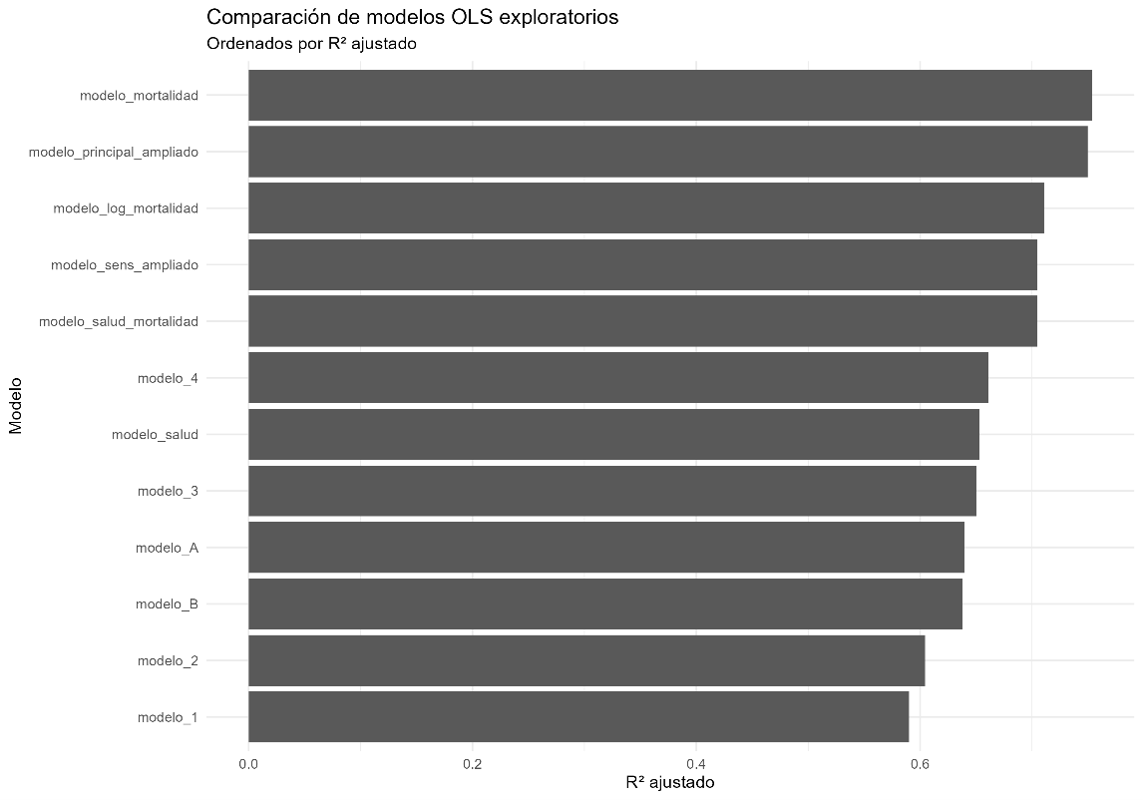
\includegraphics[width=0.65\textwidth]{fig/figures/Comparacion_OLS_exploratorios.png}
    \caption{}
\end{figure}
    \textbf{Fuente:} elaboración propia con base en estimaciones del script de modelamiento.
    
\begin{figure}[H]
    \centering
    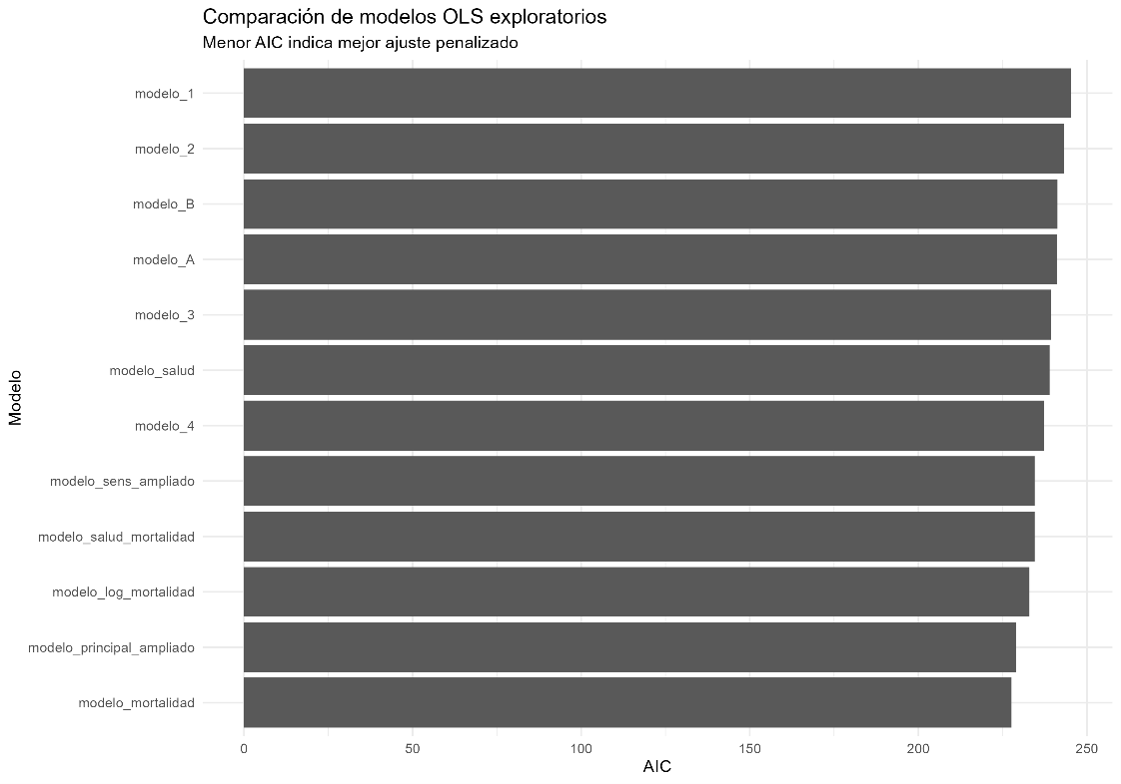
\includegraphics[width=0.65\textwidth]{fig/figures/Comparacion_OLS_exploratorios_2.png}
    \caption{}
    \textbf{Fuente:} elaboración propia con base en estimaciones del script de modelamiento.
\end{figure}

A partir de esta revisión exploratoria se seleccionaron dos especificaciones candidatas para el modelo Fay–Herriot: el modelo principal (que incluyó repitencia, infraestructura básica y mortalidad infantil) y el modelo de sensibilidad (que reemplazó la mortalidad infantil por su transformación logarítmica).

\section{Formulación del modelo Fay–Herriot}
El modelo Fay–Herriot utilizado se expresa de la siguiente manera:

\begin{equation}
    \hat{y}_d = x'_d \beta + u_d + e_d
\end{equation}

Donde $\hat{y}_d$ es la estimación directa del IPM para el departamento $d$, $x'_d$ es el vector de covariables auxiliares, $\beta$ es el vector de coeficientes, $u_d$ es el efecto aleatorio del área y $e_d$ es el error muestral asociado. Los componentes aleatorios se definen así:

\begin{align}
    u_d &\sim N(0, \sigma^2_u) \\
    e_d &\sim N(0, v_d)
\end{align}

El modelo principal se formuló como:

\begin{equation}
    \begin{split}
        IPM_d = \beta_0 + \beta_1(\text{repitencia}_d) + \beta_2(\text{infraestructura básica}_d) + \\
        \beta_3(\text{mortalidad infantil}_d) + u_d + e_d
    \end{split}
\end{equation}

El modelo de sensibilidad se formuló como:
\begin{equation}
    \begin{split}
        IPM_d = \beta_0 + \beta_1(\text{repitencia}_d) + \beta_2(\text{infraestructura básica}_d) + \\
        \beta_3[\log(1 + \text{mortalidad infantil}_d)] + u_d + e_d
    \end{split}
\end{equation}

Ambos modelos fueron ajustados mediante REML utilizando la función Fay–Herriot en R.

\section{Resultados del modelo Fay–Herriot}
Los dos modelos Fay–Herriot convergieron correctamente. No obstante, el modelo principal presentó mejores criterios de ajuste que el modelo de sensibilidad. El modelo principal obtuvo un AIC de 227,26 y un BIC de 234,75, mientras que el modelo de sensibilidad obtuvo un AIC de 232,84 y un BIC de 240,32. Por tanto, el modelo principal se adoptó como especificación de referencia para la interpretación preliminar de resultados.

En el modelo principal, los coeficientes estimados fueron consistentes con la interpretación esperada. La repitencia presentó un coeficiente positivo de 393,71, lo que indica que mayores niveles de repitencia se asocian con mayores niveles de pobreza multidimensional. La infraestructura básica presentó un coeficiente negativo de -18,48, lo que sugiere que mejores coberturas de acueducto, alcantarillado y aseo se asocian con menores niveles de IPM. La mortalidad infantil también presentó una relación positiva con el IPM, con un coeficiente de 0,12, lo cual es coherente con su interpretación como proxy de vulnerabilidad social y sanitaria del territorio.

La ecuación estimada del modelo principal se expresó como

\begin{equation}
     \begin{split}
        IPM_d = -13,84 + 393,71(\text{repitencia}_d) - 18,48(\text{infraestructura básica}_d) + \\
        0,12(\text{mortalidad infantil}_d) + u_d + e_d
    \end{split}
\end{equation}

Esta ecuación indica que, manteniendo constantes las demás variables, un aumento en la repitencia se relaciona con un incremento en el IPM; un aumento en la infraestructura básica se relaciona con una reducción en el IPM; y un aumento en la mortalidad infantil se asocia con mayores niveles de pobreza multidimensional.

En el modelo de sensibilidad, la ecuación estimada fue:

\begin{equation}
    \begin{split}
       IPM_d = -23,72 + 435,19(\text{repitencia}_d) - 21,00(\text{infraestructura básica}_d) + \\
       5,94[\log(1 + \text{mortalidad infantil}_d)] + u_d + e_d
    \end{split}
\end{equation}

Aunque el modelo de sensibilidad conservó el sentido esperado de las relaciones, presentó criterios de ajuste inferiores frente al modelo principal. Por esta razón, se mantuvo el modelo principal como referencia.

La comparación entre las estimaciones Fay–Herriot y las estimaciones directas mostró diferencias reducidas a nivel departamental (diferencia promedio de -0,038 puntos para el modelo principal), indicando un suavizamiento moderado sin cambios abruptos. En el modelo principal, la diferencia promedio entre el estimador Fay–Herriot y el IPM directo fue de -0,038 puntos, con un mínimo de -1,038 y un máximo de 1,387

\begin{figure}[H]
    \centering
    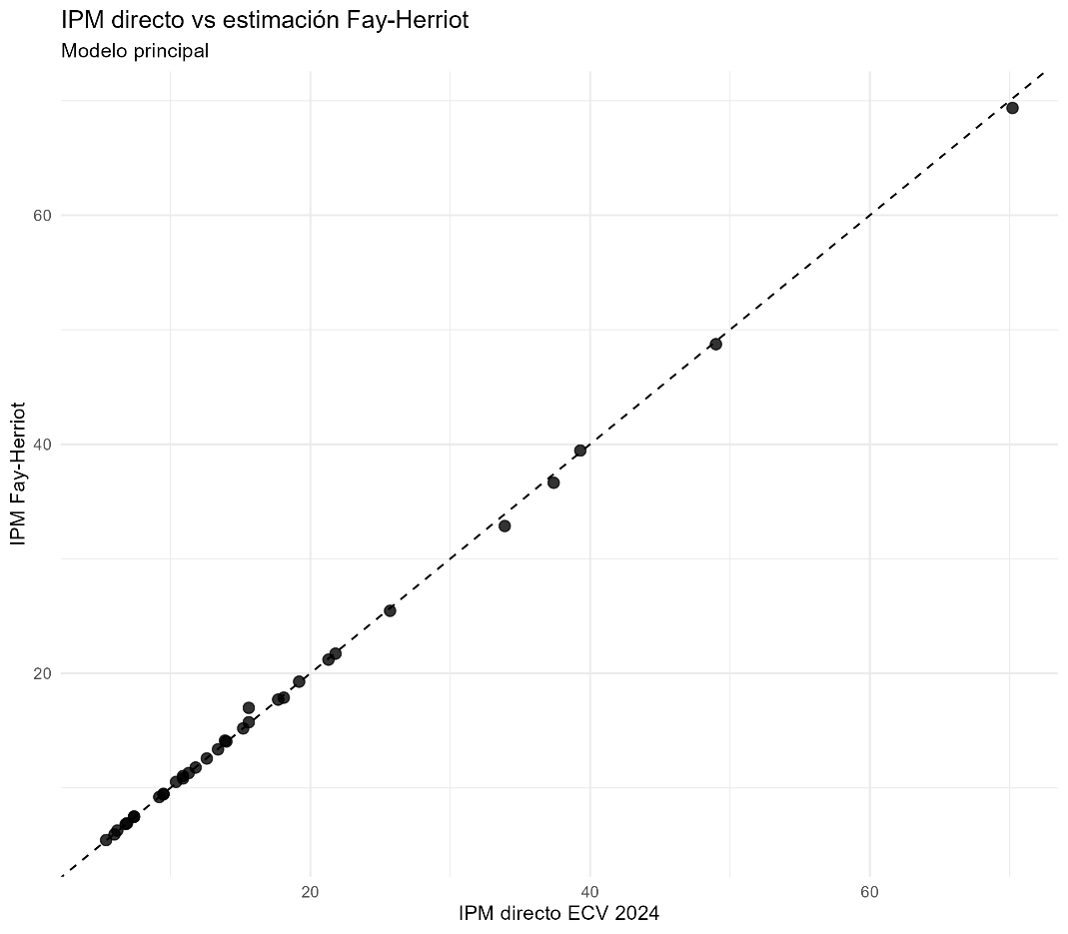
\includegraphics[width=0.65\textwidth]{fig/figures/IPM_Fay-Herriot.png}
    \caption{}
    \textbf{Fuente:} elaboración propia con base en estimaciones del script de modelamiento.
\end{figure}

La diferencia entre el modelo principal y el modelo de sensibilidad también fue reducida a nivel departamental. La diferencia promedio entre ambas estimaciones fue de -0,016 puntos, con un mínimo de -0,520 y un máximo de 0,463. Esto sugiere que, a escala departamental, las estimaciones son relativamente estables frente al cambio en la especificación de la variable de mortalidad infantil.

\begin{figure}[H]
    \centering
    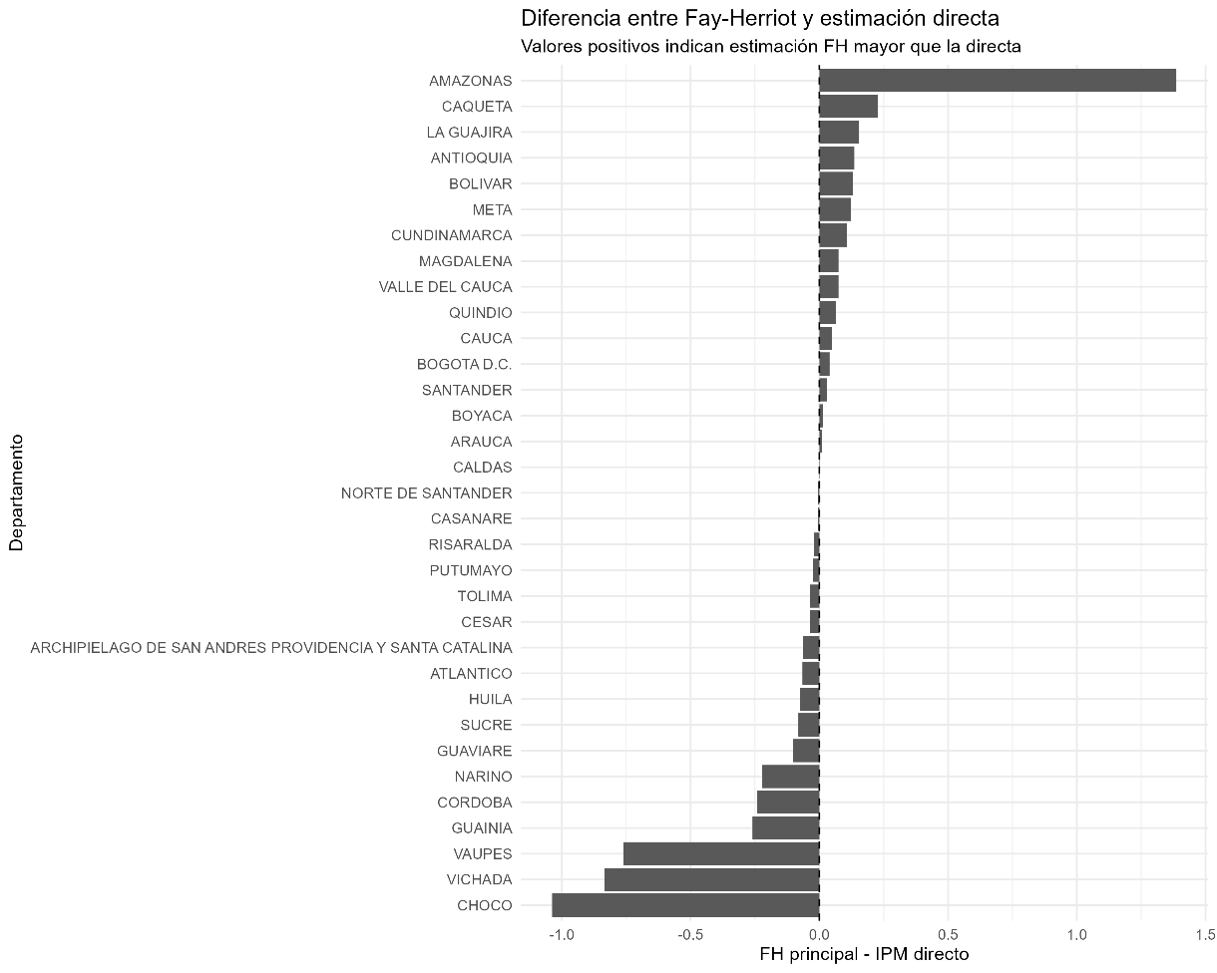
\includegraphics[width=0.65\textwidth]{fig/figures/Diferencia_Fay_Herriot-Directa.png}
    \caption{}
    \textbf{Fuente:} elaboración propia con base en estimaciones del script de modelamiento.
\end{figure}

Adicionalmente, se estimó el error cuadrático medio (MSE) del modelo Fay–Herriot. En el modelo principal, los valores de MSE se ubicaron aproximadamente entre 0,49 y 5,03, mientras que en el modelo de sensibilidad se ubicaron entre 0,49 y 5,10. Estos resultados permiten aproximar la incertidumbre asociada a las estimaciones suavizadas y constituyen un insumo relevante para comparar la precisión relativa entre departamentos.

El error estándar asociado al estimador se obtuvo mediante:

\begin{equation}
SE_{FH,d} = \sqrt{MSE_d}
\end{equation}

\begin{figure}[H]
    \centering
    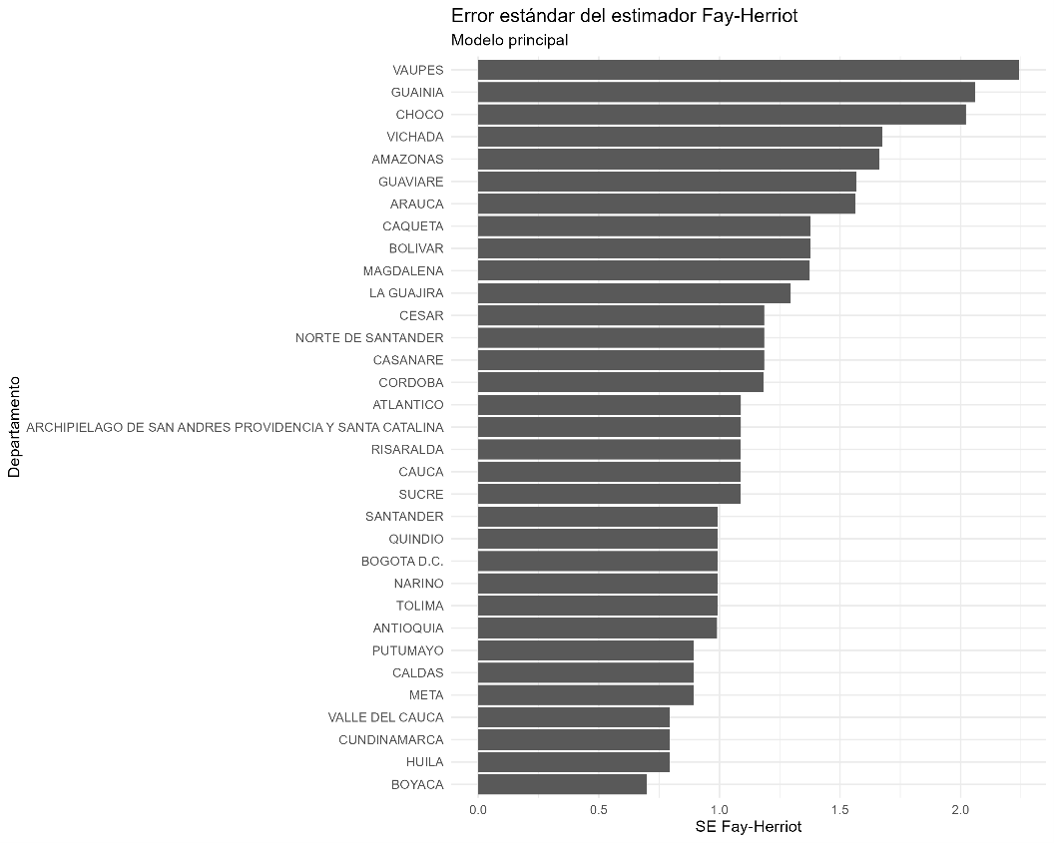
\includegraphics[width=0.65\textwidth]{fig/figures/Error_estandar_Fay-Herrot.png}
    \caption{}
    \textbf{Fuente:} elaboración propia con base en el MSE del modelo Fay–Herriot principal.
\end{figure}

\section{Predicción sintética municipal del IPM 2024}
Con base en los coeficientes estimados en los modelos Fay–Herriot, se generó una predicción sintética municipal del IPM 2024. Se aplicaron los parámetros del modelo departamental sobre la matriz de covariables municipales junto al efecto departamental estimado $\hat{u}_d$.

Las predicciones fueron acotadas entre 0 y 100 para mantener coherencia con la escala del IPM. El modelo principal se expresa entonces de manera general como:

\begin{equation}
    \begin{split}        
        IPM_{m,d} = -13,84 + 393,71(\text{repitencia}_{m,d}) - 18,48(\text{infraestructura básica}_{m,d}) \\ + 0,12(\text{mortalidad infantil}_{m,d}) + \hat{u}_d
    \end{split}
\end{equation}

Para asegurar consistencia, los resultados fueron acotados entre 0 y 100:

\begin{equation}
    IPM_{m,d}\text{ acotado} = \min[100, \max(0, IPM_{m,d})]
\end{equation}

Donde:

\begin{itemize}
    \item $IPM_{m,d}$: IPM predicho para el municipio $m$ perteneciente al departamento $d$.
    \item $\text{repitencia}_{m,d}$: repitencia del municipio $m$ en el departamento $d$.
    \item $\text{infraestructura básica}_{m,d}$: índice de infraestructura básica del municipio $m$ en el departamento $d$.
    \item $\text{mortalidad infantil}_{m,d}$: mortalidad infantil del municipio $m$ en el departamento $d$.
    \item $\hat{u}_d$: efecto departamental estimado por el modelo Fay–Herriot.
\end{itemize}

En el modelo principal, la distribución del IPM municipal predicho acotado presentó un mínimo de 0, una mediana de 10,02, una media de 13,61 y un máximo de 100. En el modelo de sensibilidad, la mediana fue de 11,86, la media de 14,91 y el rango también estuvo entre 0 y 100.

\begin{figure}[H]
    \centering
    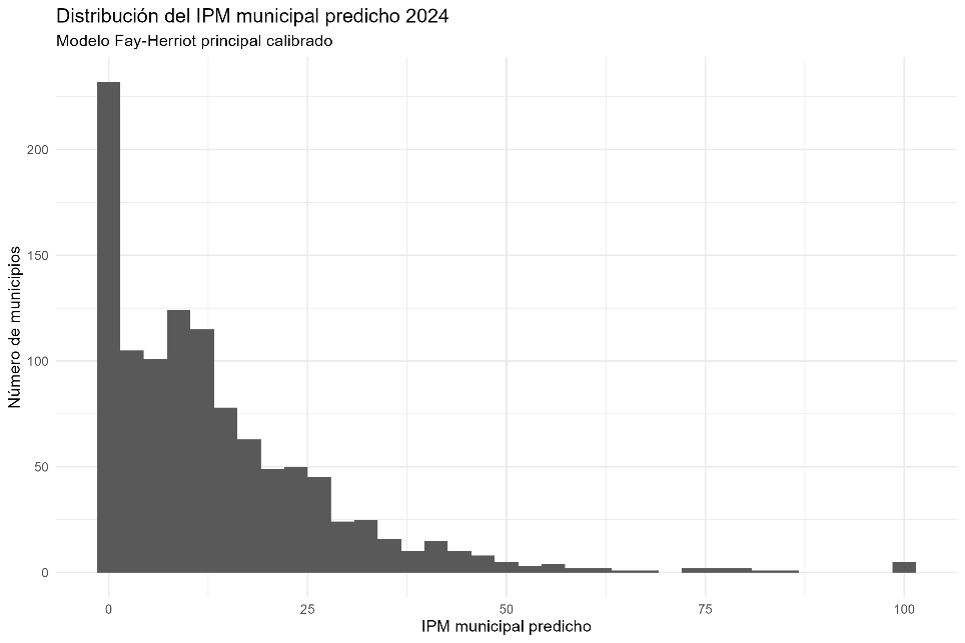
\includegraphics[width=0.65\textwidth]{fig/figures/IPM_predict_2024.png}
    \caption{}
    \textbf{Fuente:} elaboración propia con base en la comparación de predicciones municipales.
\end{figure}

La presencia de valores extremos antes del acotamiento refleja que el modelo extrapola con fuerza en algunos territorios, por lo que estas predicciones deben tomarse como un ejercicio preliminar. Por ejemplo, algunos municipios presentaron predicciones fijas superiores a 100 antes del ajuste de escala.

La diferencia entre las predicciones municipales del modelo principal y el modelo de sensibilidad se calculó como:

\begin{equation}
    \begin{split}
        \text{Diferencia}_{m,d} = \text{IPM principal}_{m,d} - \text{IPM sensibilidad}_{m,d}
    \end{split}
\end{equation}

La comparación entre el modelo principal y el modelo de sensibilidad mostró diferencias importantes en algunos municipios. Aunque la diferencia promedio entre modelos fue baja, se observaron casos con discrepancias elevadas, lo cual evidencia sensibilidad de las predicciones municipales frente a la especificación funcional de la variable de salud. Esto refuerza la necesidad de incorporar ajustes adicionales, tales como control de valores extremos, evaluación de covariables influyentes y procedimientos de calibración o benchmarking departamental.

\begin{figure}[H]
    \centering
    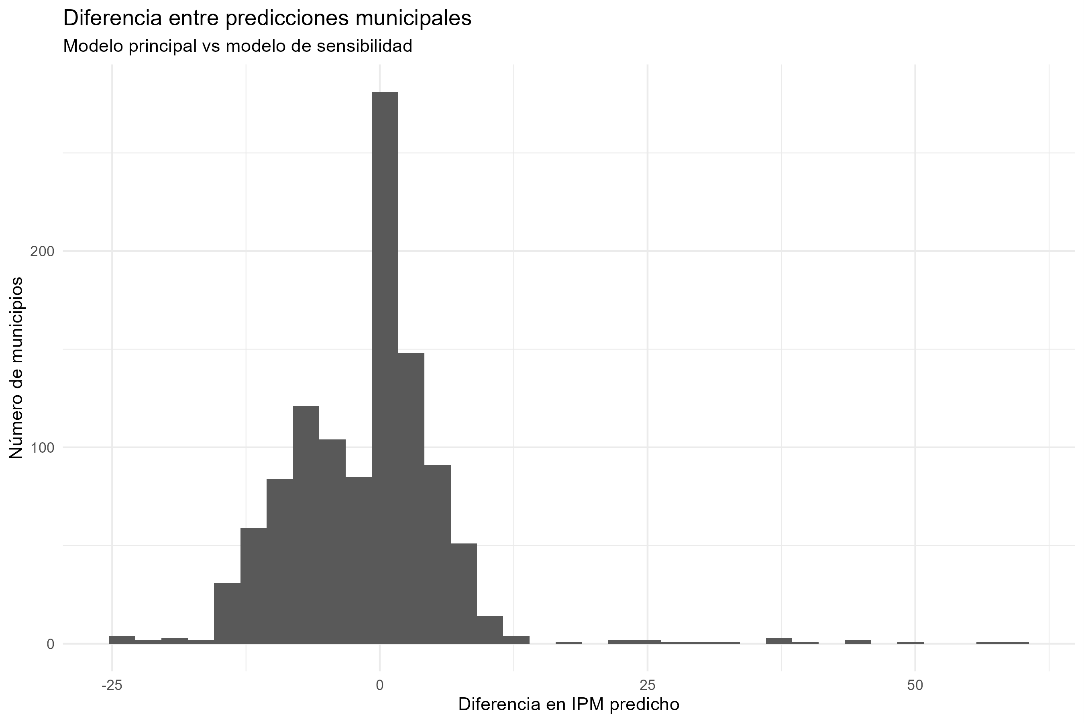
\includegraphics[width=0.65\textwidth]{fig/figures/Dif_predict_mpales.png}
    \caption{}
    \textbf{Fuente:} elaboración propia con base en la comparación de predicciones municipales.
\end{figure}

\section{Validación agregada departamental}
Como ejercicio de validación interna, se calculó el promedio del IPM municipal predicho dentro de cada departamento y se comparó con el IPM directo departamental de la ECV 2024. Esta validación no reemplaza una validación externa, pero permite evaluar si las predicciones municipales conservan la estructura territorial agregada utilizada como ancla del modelo.

El promedio municipal predicho por departamento se calculó como:

\begin{equation}
    IPM\text{ promedio}_d = \frac{1}{N_d} \sum IPM_{m,d}
\end{equation}

Los resultados arrojaron una alta correlación de 0,924 frente al IPM directo departamental de la ECV, con un RMSE de 5,36 y un MAE de 2,60. Estos valores sugieren que el modelo conserva de manera general el patrón departamental del IPM, aunque con diferencias relevantes en algunos territorios.

Las métricas formales se estructuran de la siguiente manera:

\begin{align}
    RMSE &= \sqrt{\frac{1}{D} \sum (IPM\text{ directo}_d - IPM\text{ promedio}_d)^2} 
\end{align}
\begin{align}
    MAE &= \frac{1}{D} \sum |IPM\text{ directo}_d - IPM\text{ promedio}_d|
\end{align}

Los resultados pueden apreciarse a continuación:

\begin{figure}[H]
    \centering
    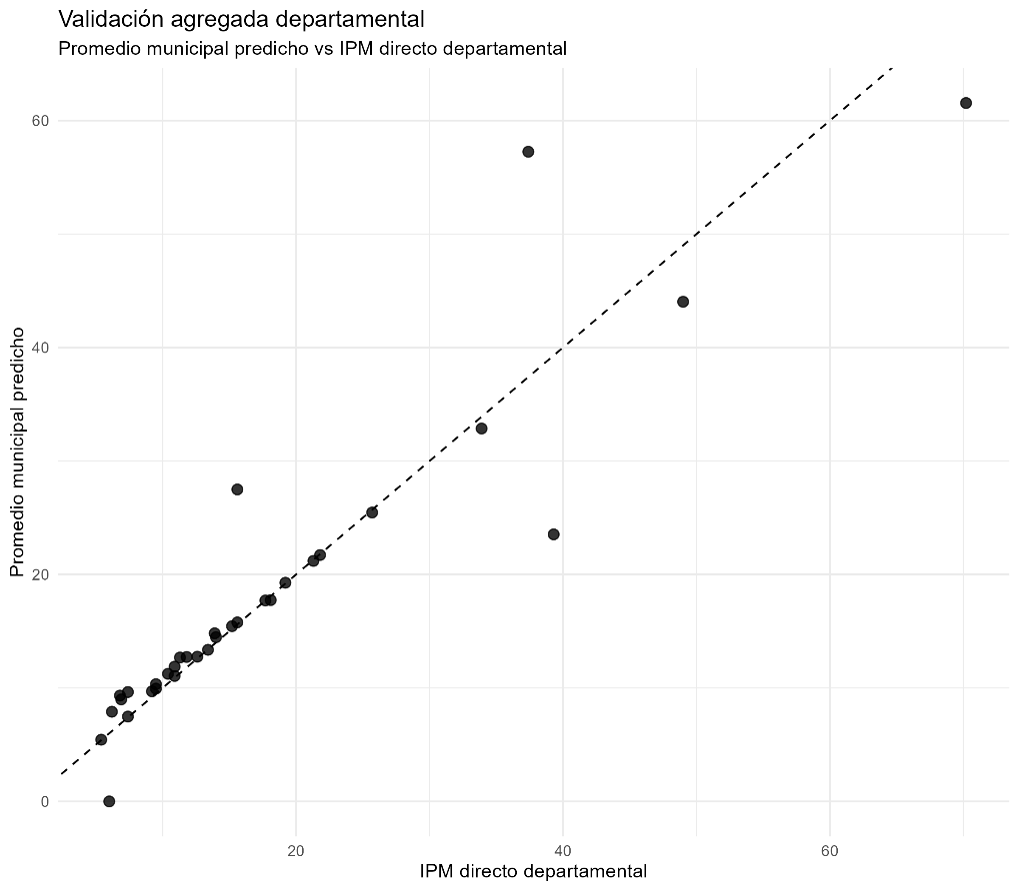
\includegraphics[width=0.65\textwidth]{fig/figures/Validacion_dptal.png}
    \caption{}
    \textbf{Fuente:} elaboración propia con base en predicciones municipales agregadas por departamento.
\end{figure}

A pesar de la alta correlación, se observaron brechas importantes en departamentos específicos como La Guajira ($-15,77$ puntos de diferencia), Amazonas ($+11,89$), Vaupés ($+19,85$), Vichada ($-8,65$) y San Andrés ($-6,00$), sugiriendo la necesidad de un proceso posterior de calibración o \textit{benchmarking}: las diferencias muestran que, aunque el modelo reproduce adecuadamente la estructura general, requiere una etapa posterior de ajuste para mejorar la coherencia entre el nivel municipal y el nivel departamental.

\section{Diagnóstico espacial preliminar}
Se aplicó la prueba global de Moran sobre los residuos de la especificación principal utilizando el criterio de contigüidad tipo reina:

\begin{equation}
    \begin{split}    
        I = \frac{D}{S_0} \frac{\sum_i \sum_j w_{ij}(e_i - \bar{e})(e_j - \bar{e})}{\sum_i (e_i - \bar{e})^2}
    \end{split}
\end{equation}

Donde:
\begin{itemize}
    \item $I$: estadístico global de Moran.
    \item $D$: número de departamentos.
    \item $w_{ij}$: peso espacial entre los departamentos $i$ y $j$.
    \item $e_i$ y $e_j$: residuos del modelo en los departamentos $i$ y $j$.
    \item $\bar{e}$: promedio de los residuos.
    \item $S_0$: suma total de los pesos espaciales.
\end{itemize}

El estadístico obtenido fue de $-0,097$ con un valor-p de $0,732$. Al ser el valor-p mayor a 0,05, no hay evidencia de auto correlación espacial positiva en los residuos departamentales, indicando que las covariables capturan satisfactoriamente la estructura territorial general. Sin embargo, debido a advertencias por discontinuidades geográficas o islas, se aconseja interpretar con cautela y explorar otras matrices de pesos.

No obstante, el procedimiento generó advertencias relacionadas con la existencia de departamentos sin vecinos y la presencia de subgrafos en la matriz de vecindad. Esto puede estar asociado a territorios insulares o a discontinuidades geográficas en la estructura departamental. Por esta razón, el diagnóstico espacial debe interpretarse con cautela y se recomienda explorar matrices de pesos alternativas, como vecinos más cercanos o criterios de distancia.

El modelo Fay–Herriot principal es consistente y conceptualmente interpretable: la repitencia se asocia al rezago educativo; la infraestructura básica refleja condiciones de vivienda y servicios; y la mortalidad infantil actúa como proxy de vulnerabilidad sanitaria. Los siguientes pasos analíticos se enfocarán en refinar la calibración municipal, corregir las predicciones en municipios atípicos y ensayar formulaciones espaciales más robustas.

%%--------------------------------------------------
%\section{Limpieza, filtrado y reglas explícitas}
   

%%--------------------------------------------------
%\section{Identificación de datos faltantes}
   


%%--------------------------------------------------
%\section{Ventanas temporales y partición de los datos en conjuntos de entrenamiento y prueba}

    
        
%%--------------------------------------------------
%\section{Construcción de variables predictoras}

    
%%--------------------------------------------------
%\section{Construcción de la variable respuesta}

    
    
%%--------------------------------------------------
%\section{Análisis exploratorio}
    
    
%%--------------------------------------------------
%\section{Preprocesamiento}


%%--------------------------------------------------
%\section{Construcción de matrices de diseño del modelo \emph{pogit}}

 
    
%%--------------------------------------------------
%\section{Reducción de dimensionalidad y segmentación ex-
%ploratoria} 


%--------------------------------------------------
%\section{Resultados de la estimación del modelo \emph{pogit}}

    
    
        
    
    % --------------------------
    \chapter{Discusión y trabajo futuro}
    \input{chapters/discusion}
   % --------------------------
    \chapter{Conclusiones}
    \input{chapters/conclusiones}
   % --------------------------
    \clearpage
    \printbibliography
    % --------------------------
     \begin{appendices}
    \chapter{Appendix}
        \input{chapters/appendice}
    \end{appendices}
\end{document}